% !TEX encoding = UTF-8
% !TEX TS-program = pdflatex
% !TEX root = ../tesi.tex

%**************************************************************
\chapter{Analisi dei requisiti}
\label{cap:analisi-requisiti}
%**************************************************************

\intro{Il presente capitolo descrive in maniera dettagliata requisiti e casi d'uso individuati durante
l'analisi del progetto di \textit{stage}.}\\

\section{Casi d'uso}
\subsubsection{Attori pricipali}
Nell'analisi del progetto di \textit{stage} è emerso solo un attore, ovvero l'\textbf{utente autenticato}, 
attore che indica un utente che ha effettuato l'autenticazione
all'interno dell'applicazione web. Ha quindi la possibilità di vedere tutte le
informazioni sui gruppi e sulle \gls{will}  che sarebbero altrimenti inaccessibili. 

\subsubsection{Elenco dei casi d'uso}
Per lo studio dei casi di utilizzo del prodotto sono stati creati dei diagrammi.
I diagrammi dei casi d'uso (in inglese \emph{Use Case Diagram}) sono diagrammi di tipo \gls{uml} dedicati alla descrizione delle funzioni o servizi offerti da un sistema, così come sono percepiti e utilizzati dagli attori che interagiscono col sistema stesso.
\begin{figure}[H] 
    \centering 
    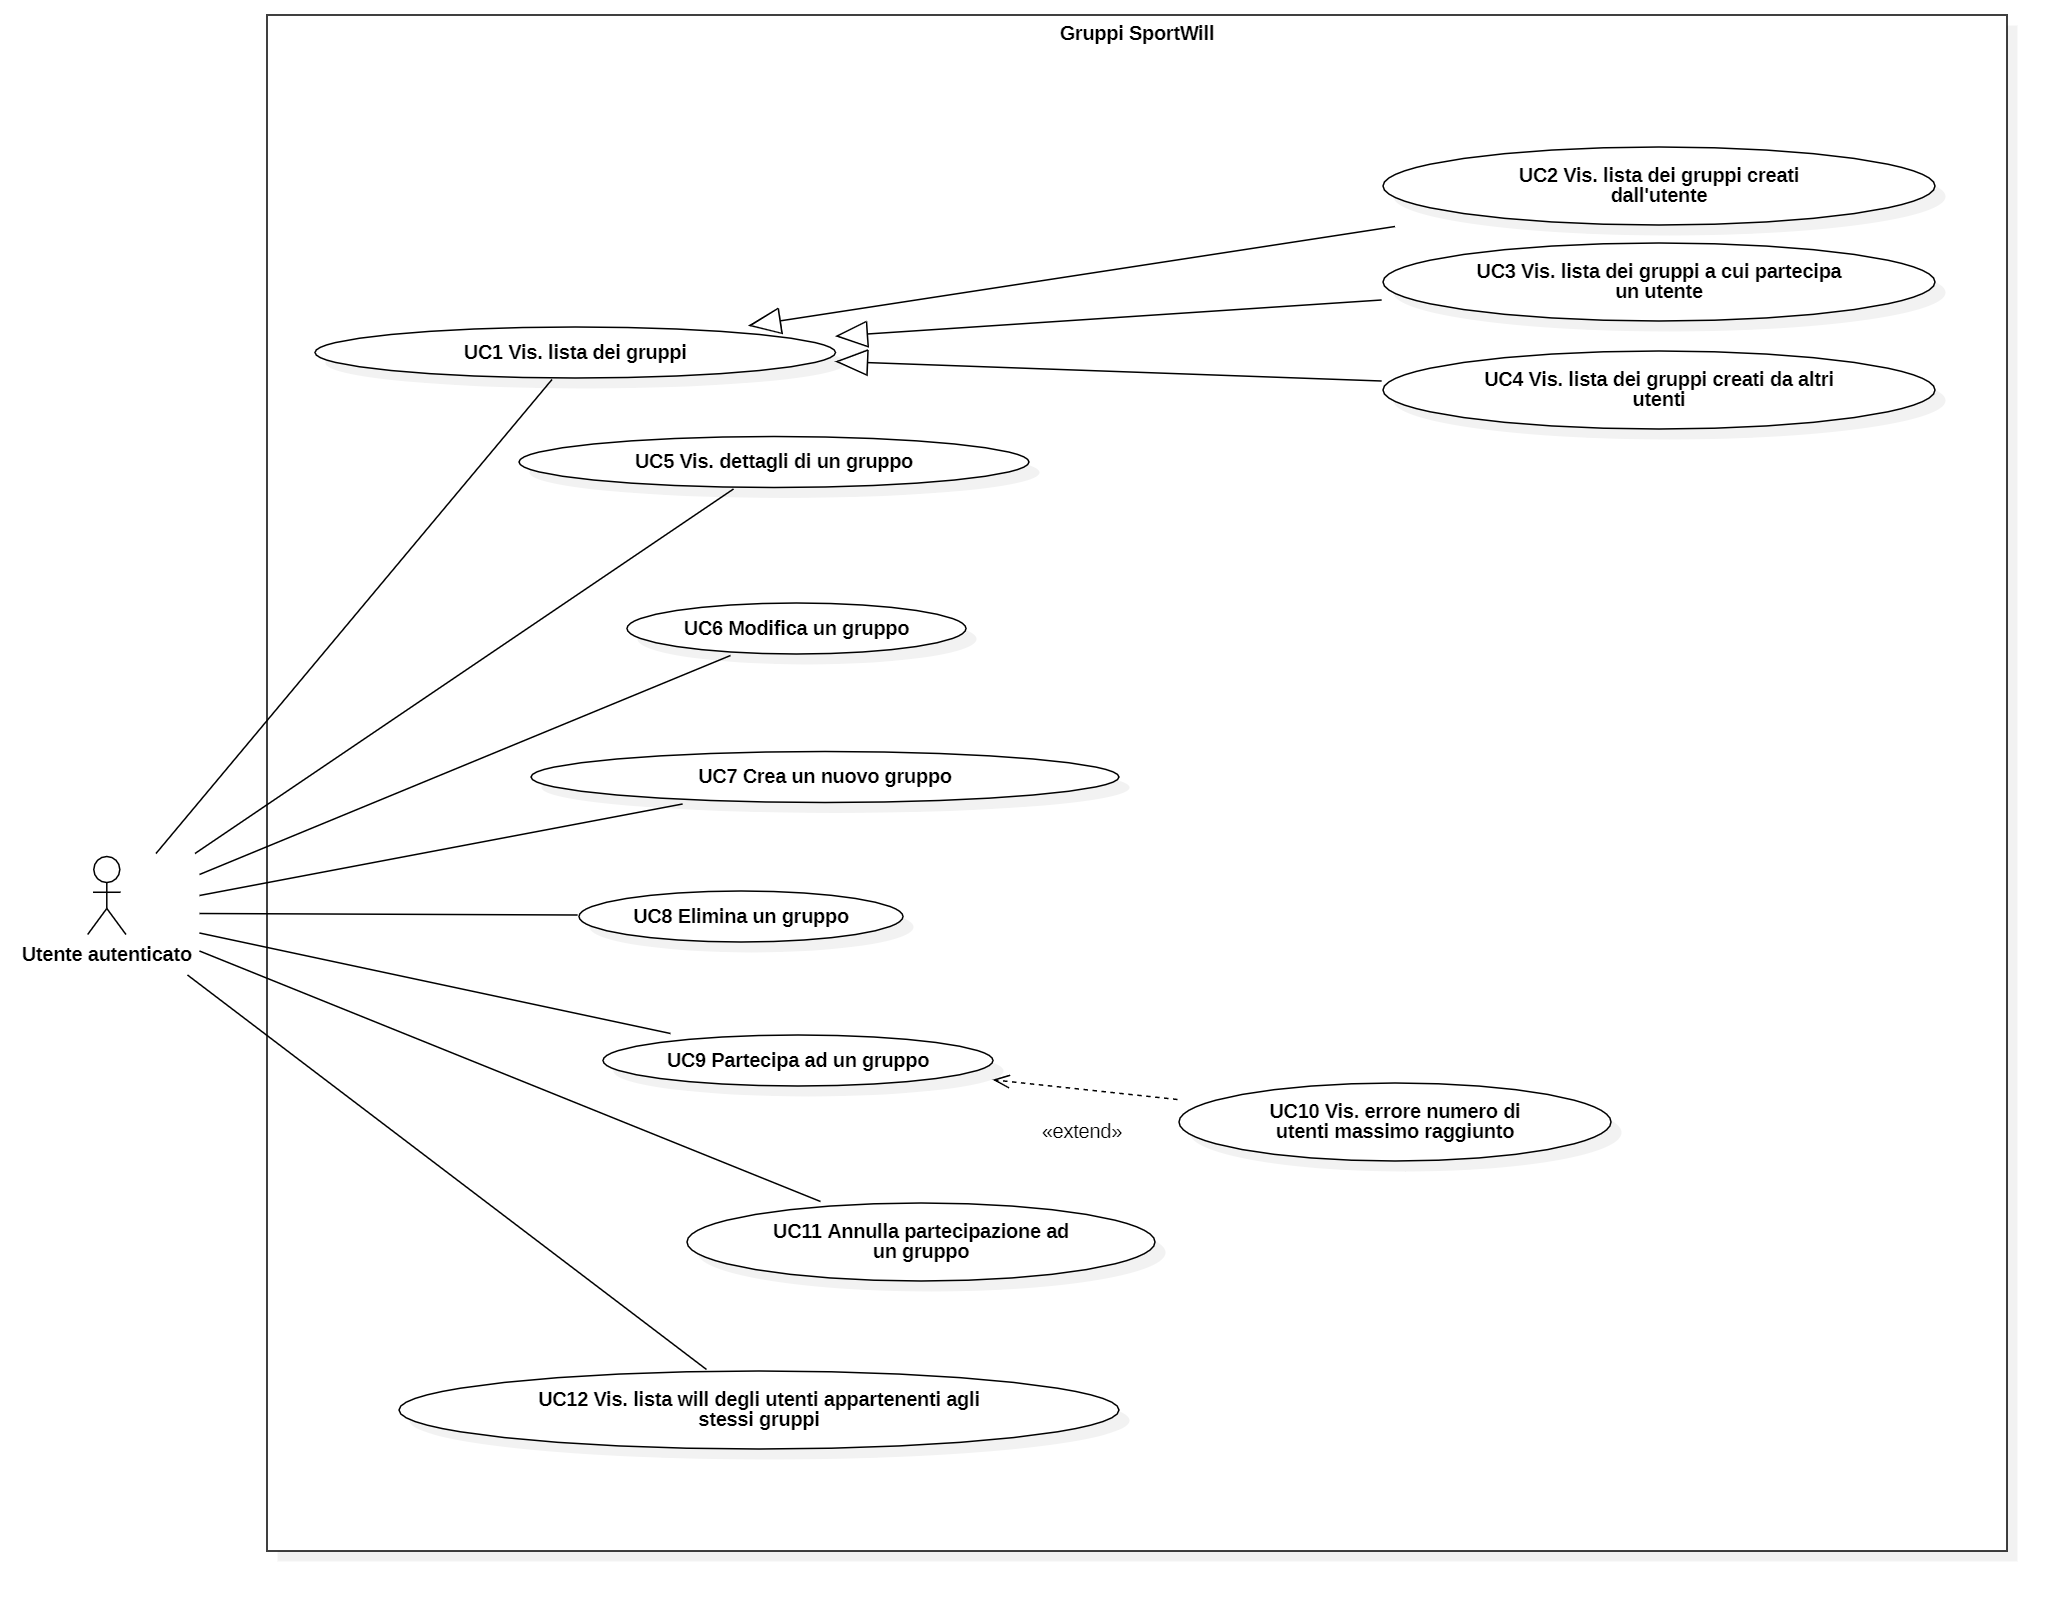
\includegraphics[width=1.2\columnwidth]{usecase/diagramma generale dei casi d'uso.png} 
    \caption{Use Case - UC0: Scenario principale}
\end{figure}

\begin{usecase}{Prova2}
    \usecaseactors{Sviluppatore applicativi}
    \usecasepre{Lo sviluppatore è entrato nel plug-in di simulazione all'interno dell'IDE}
    \usecasedesc{La finestra di simulazione mette a disposizione i comandi per configurare, registrare o eseguire un test}
    \usecasepost{Il sistema è pronto per permettere una nuova interazione}
    \label{uc:scenario-due}
\end{usecase}

\begin{usecase}{Prova1}
    \usecaseactors{Sviluppatore applicativi}
    \usecasepre{Lo sviluppatore è entrato nel plug-in di simulazione all'interno dell'IDE}
    \usecasedesc{La finestra di simulazione mette a disposizione i comandi per configurare, registrare o eseguire un test}
    \usecasepost{Il sistema è pronto per permettere una nuova interazione}
    \label{uc:scenario-principale}
    \end{usecase}

\section{Tracciamento dei requisiti}

Da un'attenta analisi dei requisiti e degli use case effettuata sul progetto è stata stilata la tabella che traccia i requisiti in rapporto agli use case.\\
Sono stati individuati diversi tipi di requisiti e si è quindi fatto utilizzo di un codice identificativo per distinguerli.\\
Il codice dei requisiti è così strutturato R(F/Q/V)(N/D/O) dove:
\begin{enumerate}
	\item[R =] requisito
    \item[F =] funzionale
    \item[Q =] qualitativo
    \item[V =] di vincolo
    \item[N =] obbligatorio (necessario)
    \item[D =] desiderabile
    \item[Z =] opzionale
\end{enumerate}
Nelle tabelle \ref{tab:requisiti-funzionali}, \ref{tab:requisiti-qualitativi} e \ref{tab:requisiti-vincolo} sono riassunti i requisiti e il loro tracciamento con gli use case delineati in fase di analisi.

\newpage

\begin{table}%
\caption{Tabella del tracciamento dei requisti funzionali}
\label{tab:requisiti-funzionali}
\begin{tabularx}{\textwidth}{lXl}
\hline\hline
\textbf{Requisito} & \textbf{Descrizione} & \textbf{Use Case}\\
\hline
RFN-1     & L'interfaccia permette di configurare il tipo di sonde del test & UC1 \\
\hline
\end{tabularx}
\end{table}%

\begin{table}%
\caption{Tabella del tracciamento dei requisiti qualitativi}
\label{tab:requisiti-qualitativi}
\begin{tabularx}{\textwidth}{lXl}
\hline\hline
\textbf{Requisito} & \textbf{Descrizione} & \textbf{Use Case}\\
\hline
RQD-1    & Le prestazioni del simulatore hardware deve garantire la giusta esecuzione dei test e non la generazione di falsi negativi & - \\
\hline
\end{tabularx}
\end{table}%

\begin{table}%
\caption{Tabella del tracciamento dei requisiti di vincolo}
\label{tab:requisiti-vincolo}
\begin{tabularx}{\textwidth}{lXl}
\hline\hline
\textbf{Requisito} & \textbf{Descrizione} & \textbf{Use Case}\\
\hline
RVO-1    & La libreria per l'esecuzione dei test automatici deve essere riutilizzabile & - \\
\hline
\end{tabularx}
\end{table}%